\subsection*{2.1a}
The parameters that were experimented with (independently) were the 
learning rate (0.0002, 0.002, 0.02), as this
can schedule what performance can be reached under different levels learning rate. Furthermore,
the sequence length of our data was tested (30, 60, 80), as shown earlier, to test how well it performs
on longer dependencies. Finally, also differnet amount of layers are tested(1,2,3) as well as number of hidden neuron (64,128,256). 
These were chosen simply to test the effect of deeper / wider LSTM networks.
Finally, this was trained primarily on the provided Democracy in the US book. The optimal paramters (independently) were
found to be $lr=0.02, seqlength=30, nrlayers=2, nrhidden=256$, which was run separately al-together. However, it is important to note that within the same dataset,
given sufficient training time, the differnece in training is neglible, and learning-rate becomes the most essential parameter.
Because of this, any figure would show similar pattern, converging sooner or later at around an Accuracy of 0.65.

\begin{figure}%
    \centering
    \subfloat[\centering Accuracy for best model]{{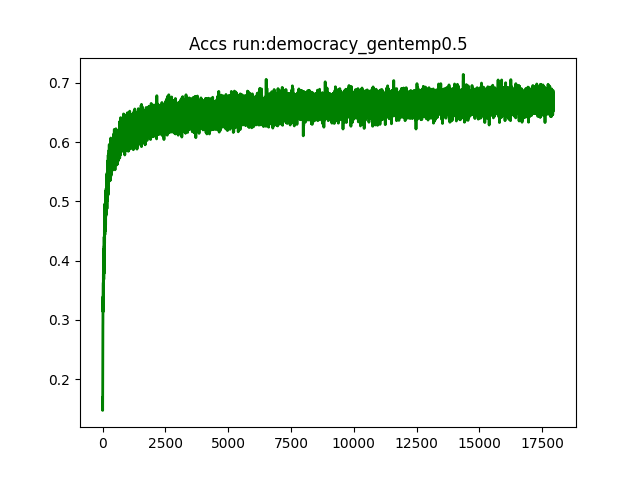
\includegraphics[width=6.5cm]{images/training-plots-accs.png} }}%
    \qquad
    \subfloat[\centering Loss for best model]{{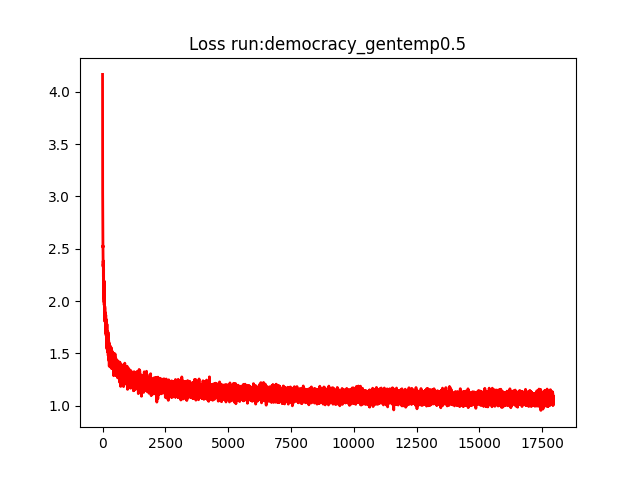
\includegraphics[width=6.5cm]{images/training-plots-loss.png} }}%
    \caption{Loss and accuracy for best model}%
    \label{fig:defaults}%
\end{figure}

\subsection*{2.1b}
\noindent\fbox{%
    \parbox{\textwidth}{%
    LEN=30


    After seeing 100 samples (starting with J)
    J on the the the the the the t
    
    After seeing 3900 samples (starting with 6)
    60,000 miles of the Union the 
    
    RAfter seeing 12000 samples (starting with R)
    Republican courts of the State
    
    After seeing 16000 samples (starting with X)
    XVIII: Future Condition is alw
    
    
    AFter seeing 18000 samples (starting with Y)
    You may be adopted by the cont
    
    LEN=50
    
    Seeing 100 samples (starting with J)
    Gthe the the the the the the the the the the the t
    
    Seeing 3900 samples (starting with g)
    great an individual and the present the present th
    
    Seeing 12000 samples (starting with W)
    When the principal constitution of the United Stat
    
    Seeing 16000 samples (starting with t)
     the principle of the United States the same power

     LEN=20

    Seeing 99 samples (seeing Q): Qrrrrr

    Seeing 3900 samples (seeing I): In the United States

    Seeing 12000 samples (seeing J): Jects of the country

    Seeing 16000 samples (seeing 6): 6, and the present t

    Seeing 18000 samples (seeing V): Vigrania is the cons
}
}

In above box, a few sentense excerpts are picked apart, based on previously
"best" model trained on the Democracy in the US book. What became very apparent
during running and generating sentence, is a strong and clear bias for particular
phrases (principal, United States, principle, constitution, country). Some of these
excerpt project that, but this becomes more paprent with logner sentences, as the
model has a higher likelihood to generate onf oits biases. Fortunately, after 1000 iterations or so,
the model becomes successful at generating readable and coherent sentences (even if somewhat repetitive). 
However, no mattter how readable, it is clear that the logner sentences get, the more the model seems to have the
tendency to repeat certain phrases (great an individual and the present the present). These phrases seem to be most
typical and indicative of this dataset, so if these words were to be reweighed, it might be possible
that more unique sentences could be generated.

\subsection*{2.1c}
Temperature is added to the exponents in a softmax to "punish" larger numbers more. 
What that essentially means, is that the original probabilities in favour of common words (such as "United States") previously
should get scaled back a little bit, and allow the network to make slightly less predictable predictions. However, important to note
is that in this case, we use the 'inverted' temperature $(1/T)$, so the lower temperature, the more high probabilities get punished.
When applied to the democracy dataset using the same settings as were chosen in the previous example, we can absolutely recognize this in the 
generated sentences:

\noindent\fbox{%
    \parbox{\textwidth}{
        For example, these are the sentences that are sampled for our "democracy" data-set:

        Temperature 2

        - Majority which are
        - 0 from the law with the admin
        - European nations
        - Zenehwer the exerciss

        Temperature 0.5

        - lafue loat, asing tadelent has
        - Q Fedent parvey, nome. From
        ways yir thellet, ... hanized

        For the dutch dataset about Darwin's travels around the world:

        Temperature 2:
        - pleken wij daarop het hoofd do
        - in den grond niet gescheiden
        - p van de boomen en schildwacht
        - één klein manier is met de

        Temperature 0.5:

        - kogla melf, Lier noindent
        - Fraai. Eenkel
        - äwonia 20:
        - Oze fron, Wnaslage Nuargo
    }
}

These sentences show the difference in temperature more than enough. Both for the English and Dutch language,
a low temperature produces nonsenical but syntactically similar sentences. The vocabulary is non-existant,
but the usage of punctuation works similar to the more coherent (but boring) predictions when temperature = 2. 
Greedy sampling, however, was most predictable, as it seemed as if sentences somehow kept reocccuring, even if only paraphrased.